\chapter{\scshape Requisiti e Progettazione Architetturale}

\section{Analisi delle criticità pregresse e requisiti}\label{cap:2.1-criticita}
La progettazione del software end-to-end per l'autenticazione biometrica remota tramite documento d'identità, in oggetto di questa tesi, ha preso avvio da un'analisi approfondita di un \textbf{precedente prototipo} di verifica dell'identità, al fine di individuarne i limiti strutturali, le vulnerabilità e i colli di bottiglia prestazionali.
Il primo elemento di criticità riscontrato riguardava la calibrazione della soglia decisionale di somiglianza coseno, originariamente fissata a un \textbf{valore estremamente permissivo} ($\tau = 0{,}15$). Come discusso nel Capitolo~\ref{cap:1-fondamenti}, una soglia così bassa nei modelli basati su margine angolare additivo come \gls{arcface}, azzera apparentemente il tasso di falsi rifiuti (\textit{False Reject Rate}) ma, al contempo, aumenta drasticamente il tasso di falsi accettati (\textit{False Accept Rate}), rendendo il sistema vulnerabile a tentativi di impersonificazione tramite \textit{spoofing}~\cite{azizFaceRecognitionBase2024}.
Una seconda carenza strutturale risiedeva nella \textbf{totale assenza} di una pipeline di pre-elaborazione dedicata al documento d'identità. Tentare l'estrazione diretta del volto da una fotografia grezza della \gls{cie} senza prima correggere le distorsioni prospettiche d'inquadratura e migliorare il contrasto, espone il modello al degrado tipico del \textit{cross-domain matching}, causando frequenti fallimenti nello stadio di \textit{face detection} o la generazione di vettori di embedding fortemente rumorosi~\cite{fangIDCardIdentification2017,caldeiraImpactFaceSegmentationBased2026}.
A ciò si aggiungeva \textbf{l'inaffidabilità del modulo \gls{pad}}: si faceva affidamento su componenti aggiuntivi instabili basati su versioni obsolete di \textit{PyTorch} operando, inoltre, in maniera \textit{stateless} su singoli fotogrammi isolati~\cite{liSilentFaceAntiSpoofing2024}.
L'assenza di una validazione temporale su un buffer di frame, rendeva il sistema vulnerabile a semplici attacchi di presentazione \textit{print attacks} e \textit{replay attacks}, con conseguenti falsi rifiuti \textit{\gls{bpcer}} e accettazione di attacchi \textit{\gls{apcer}}, innescati da variazioni di illuminazione, posa o artefatti di \textit{motion blur}~\cite{azizFaceRecognitionBase2024}.

Oltre alle vulnerabilità strettamente algoritmiche, l'architettura pregressa presentava severi limiti sotto il profilo dell'ingegneria del software, della scalabilità e della conformità normativa.
In primo luogo, il prototipo analizzato era privo di uno strato di persistenza multi-utente strutturata. L'assenza di un database capace di indicizzare i vettori biometrici impediva la gestione concorrente di molteplici identità registrate e non consentiva di separare logicamente la fase di registrazione \textit{enrollment} da quella di autenticazione.
Dal punto di vista computazionale, la gestione dei modelli di \textit{deep learning} risultava inefficiente: i pesi dei modelli venivano caricati in memoria RAM ad ogni utilizzo, anziché pre-caricarli in anticipo, causando un overhead di latenza e un consumo eccessivo di risorse CPU/RAM, con conseguente degrado delle prestazioni.
Sotto il profilo della sicurezza dei dati, la gestione dei file temporanei salvati sul disco locale violava i principi di \textit{minimizzazione dei dati} e \textit{limitazione della conservazione} previsti dalla normativa discussa nel Capitolo~\ref{cap:1.4-normative}, esponendo i dati biometrici grezzi a rischi di furto o profilazione non autorizzata, in violazione del GDPR e dell'AI Act~\cite{sanzGoverningPrivacyPreservingFace2026}.
La Tabella~\ref{tab:confrontoLegacyNuovo} sintetizza le criticità analizzate mettendole a confronto con le soluzioni progettate nel nuovo sistema.
\begin{table}[H]
    \centering
    \footnotesize
    %\begin{tabular}{c c c c}
    \begin{tabular*}{\textwidth}{@{\extracolsep{\fill}} >{\raggedright\arraybackslash}p{3.0cm} >{\raggedright\arraybackslash}p{5.2cm} >{\raggedright\arraybackslash}p{5.4cm} @{}}
        \hline
        \textbf{Ambito di Analisi} & \textbf{Criticità Prototipo Pregresso} & \textbf{Soluzione Adottata} \\
        \hline
        \textbf{Soglia di Matching} & Soglia troppo permissiva ($\tau = 0{,}15$), con conseguente \gls{far} critico e accettazione di impostori & Calibrazione della soglia ($\tau \in [0{,}30, \, 0{,}50]$) per bilanciare sicurezza (\gls{far}) e usabilità (\gls{frr}) \\
        %\hline
        \textbf{Acquisizione \gls{cie}} & Assenza di pre-processing sul documento; estrazione diretta sensibile a prospettiva e basso contrasto. & Pipeline geometrica e ottica dedicata con rettifica prospettica (\textit{warp}) ed equalizzazione locale \gls{clahe} \\
        %\hline
        \textbf{Liveness Detection} & Modulo passivo instabile o basato su dipendenze obsolete, eseguito su singolo frame isolato & Rete leggera \textit{MiniFASNet} su \gls{onnx} Runtime ($\sim 1~\text{MB}$) combinata con analisi su buffer temporale e tracciamento dei 5 keypoint~\cite{liSilentFaceAntiSpoofing2024}. \\
        %\hline
        \textbf{Persistenza e Privacy} & Assenza di database multi-utente e salvataggio temporaneo delle immagini su disco locale & Database vettoriale \textit{MongoDB Atlas Vector Search} e politica \textit{Zero-Disk Retention}~\cite{sanzGoverningPrivacyPreservingFace2026}. \\
        %\hline
        \textbf{Esperienza Utente} & Mancanza di supporto interattivo & Applicazione web multipiattaforma (\gls{pwa}) con acquisizione della \gls{cie} e feedback in tempo reale \\
        \hline
    %\end{tabular}
    \end{tabular*}
    \caption{Confronto tra le criticità riscontrate nel prototipo pregresso e le soluzioni introdotte nella nuova architettura realizzata.}~\label{tab:confrontoLegacyNuovo}
\end{table}

Sulla base delle evidenze raccolte e dei vincoli teorico-normativi esposti nel capitolo~\ref{cap:1-fondamenti}, si è proceduto alla specifica formale dei requisiti della nuova piattaforma software.
I requisiti sono stati classificati secondo lo standard dell'ingegneria del software in:
\begin{itemize}
    \item \textbf{\gls{rf}}: descrivono le funzionalità che il sistema deve implementare, le interazioni che il sistema deve offrire agli utenti e i flussi di elaborazione biometrica;
    \item \textbf{\gls{rnf}}: descrivono le caratteristiche qualitative del sistema, come la scalabilità, le prestazioni in tempo reale, la sicurezza dei dati, la latenza di rete, l'ottimizzazione delle risorse e la tutela della privacy.
\end{itemize}
Sul piano funzionale, il sistema deve supportare due flussi operativi principali: \textit{enrollment} e \textit{live verification}. 
Il flusso di \textbf{\textit{enrollment}} consente la registrazione di un nuovo utente, acquisendo la fotografia del documento conforme allo standard ICAO 9303 formato TD1, da cui estrarre e indicizzare il template di riferimento nel database. Si è scelto di evitare la scansione del retro per minimizzare l'attrito nella \gls{ux}, richiedendo all'utente di inserire il suo nominativo. Inoltre, si effettuano i \textbf{controlli di unicità} per impedire la registrazione di più identità associate allo stesso soggetto biometrico.
La fase di \textbf{\textit{live verification}} consente invece la verifica dell'identità di un utente già registrato, acquisendo un flusso video in tempo reale dalla fotocamera del dispositivo, sottoponendolo a verifica di vitalità e confrontando il volto rilevato con i vettori archiviati nel database per determinare l'identità del soggetto.
\\Sul piano \textbf{non funzionale}, l'architettura deve garantire un budget di latenza sub-secondo per l'elaborazione dei singoli frame video, l'isolamento crittografico delle comunicazioni di rete e l'assoluta aderenza al paradigma \textit{Zero-Disk Retention}, evitando la persistenza su disco dei dati biometrici grezzi e dei fotogrammi acquisiti.
In Figura~\ref{fig:diagrammaCasiDuso} è riportato il diagramma dei casi d'uso UML del sistema progettato, che illustra le interazioni tra l'utente e i flussi operativi di \textit{enrollment} e \textit{live verification}.
\begin{figure}[H]
    \centering
    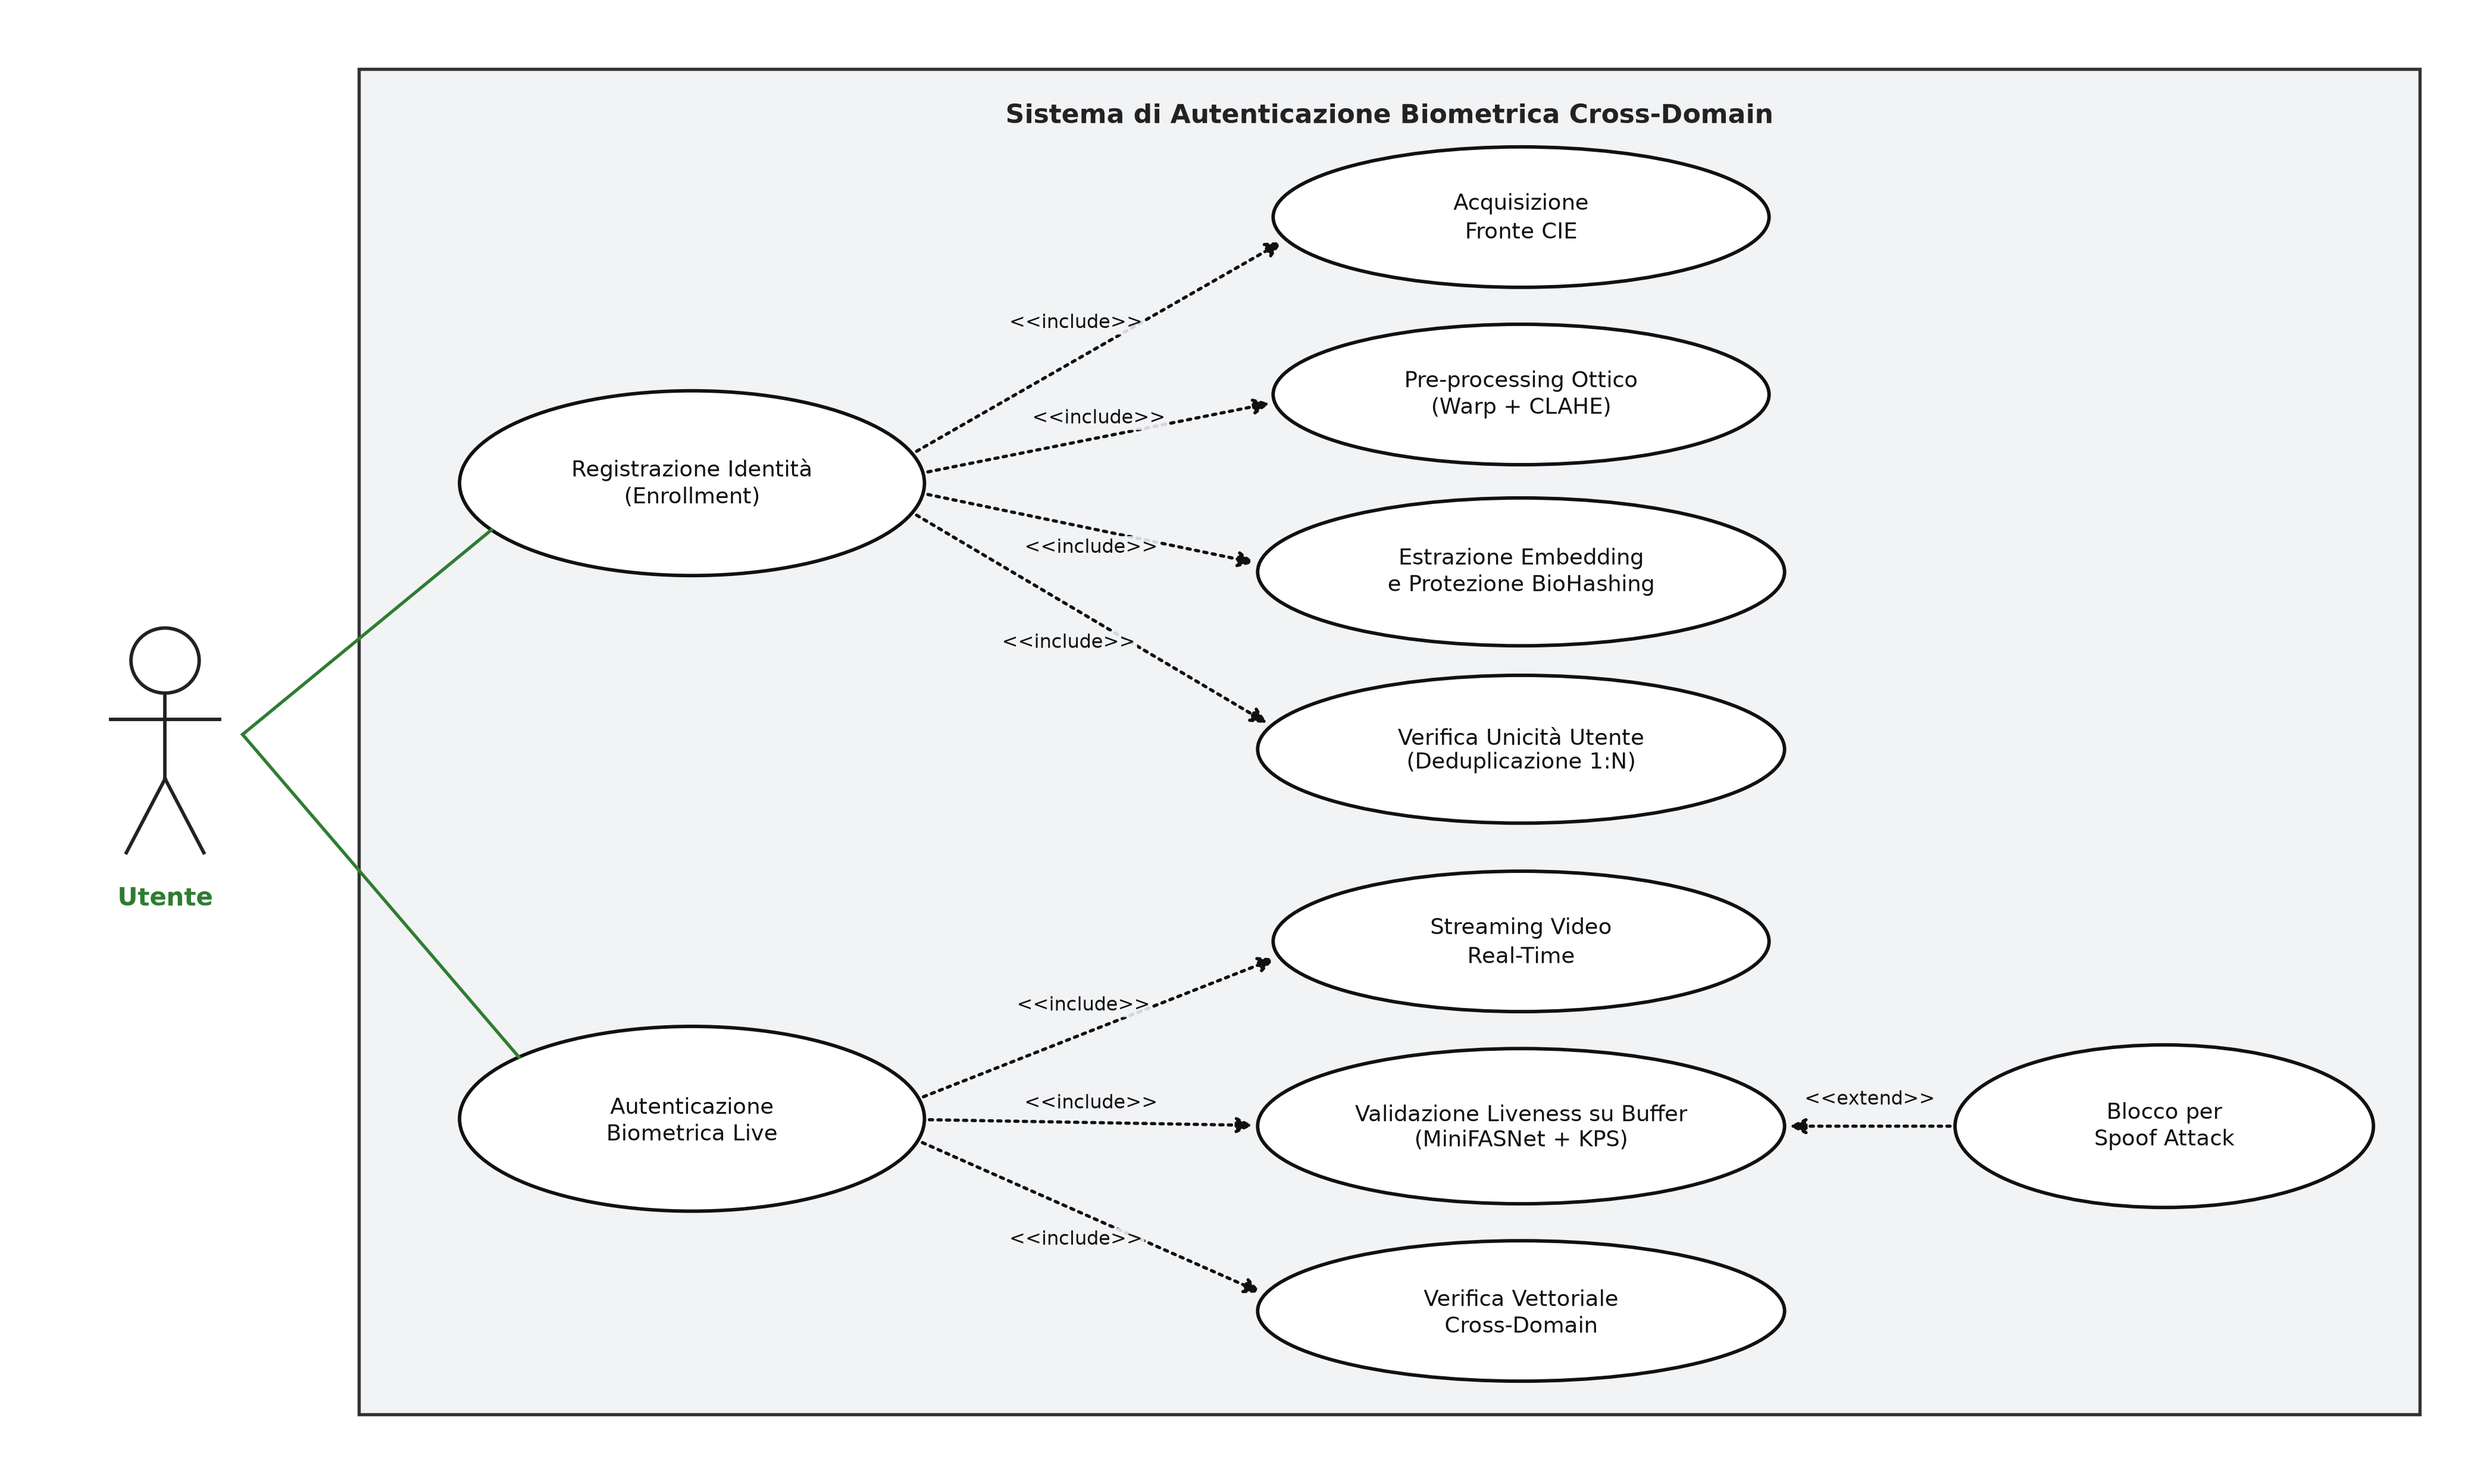
\includegraphics[width=\textwidth]{images/diagramma-casi-duso.png}
    \caption{Diagramma dei Casi d'Uso UML del sistema di autenticazione biometrica.}\label{fig:diagrammaCasiDuso}
\end{figure}
Nelle tabelle~\ref{tab:requisitiFunzionali} e~\ref{tab:requisitiNonFunzionali} sono riportati rispettivamente l'elenco completo e strutturato dei requisiti funzionali e non funzionali del progetto, con le relative priorità secondo la metodologia \textit{\gls{moscow}}.
\begin{table}[H]
    \centering
    \footnotesize
    \renewcommand{\arraystretch}{1.25}
    %\begin{tabular}{c c c c}
    \begin{tabular*}{\textwidth}{@{\extracolsep{\fill}} c >{\raggedright\arraybackslash}p{3.4cm} >{\raggedright\arraybackslash}p{7.4cm} c @{}}
        \hline
        \textbf{ID} & \textbf{Requisito} & \textbf{Descrizione} & \textbf{Priorità} \\
        \hline
        RF1 & Acquisizione e Pre-processing \gls{cie} & Il sistema deve acquisire il lato anteriore di un documento ICAO TD1, applicando rettifica prospettica e miglioramento del contrasto locale (\gls{clahe}). & \textit{Must} \\
        \hline
        RF2 & Estrazione Deep Face Embedding & Il sistema deve rilevare e allineare il volto sui 5 keypoint biometrici, estraendo un vettore normalizzato $e \in \mathbb{R}^{512}$ ($\lVert e \rVert_2 = 1$). & \textit{Must} \\
        \hline
        RF3 & Liveness Detection Multi-Frame & Il sistema deve validare la presenza biologica reale su un buffer temporale di fotogrammi, combinando lo score passivo di \textit{MiniFASNet} e l'analisi di movimento dei keypoint. & \textit{Must} \\
        \hline
        RF4 & Matching Vettoriale Multi-Utente & Il sistema deve confrontare l'embedding \textit{live} con i template registrati nel database vettoriale mediante \textit{Cosine Similarity} e soglia calibrata ($\tau \ge 0{,}30$). & \textit{Must} \\
        \hline
        RF5 & Unicità di Registrazione (Deduplicazione) & In fase di registrazione (\textit{enrollment}), il sistema deve eseguire una ricerca vettoriale $1:N$ per impedire che lo stesso soggetto biometrico venga associato a più identità distinte & \textit{Must} \\
        \hline
        RF6 & Guida Interattiva Real-Time & L'interfaccia client deve fornire feedback visivi in tempo reale sullo stato della sessione (attesa volto, avanzamento buffer liveness, esito verifica) & \textit{Should} \\
        \hline
    %\end{tabular}
    \end{tabular*}
    \caption{Specifica formale dei Requisiti Funzionali (RF) del sistema progettato.}
    \label{tab:requisitiFunzionali}
\end{table}

\begin{table}[H]
    \centering
    \footnotesize
    \renewcommand{\arraystretch}{1.25}
    %\begin{tabular}{c c c c}
    \begin{tabular*}{\textwidth}{@{\extracolsep{\fill}} c >{\raggedright\arraybackslash}p{3.4cm} >{\raggedright\arraybackslash}p{7.4cm} c @{}}
        \hline
        \textbf{ID} & \textbf{Requisito} & \textbf{Descrizione} & \textbf{Priorità} \\
        \hline
        RNF1 & Bassa Latenza (Prestazioni) & I modelli neurali devono risiedere pre-allocati in memoria RAM, garantendo tempi di inferenza per singolo frame nell'ordine di $30{-}50~\text{ms}$ & \textit{Must} \\
        \hline
        RNF2 & Zero-Disk Retention (Privacy) & Le scansioni dei documenti e i fotogrammi video devono essere elaborati esclusivamente in memoria volatile (RAM) e distrutti istantaneamente dopo l'estrazione del vettore & \textit{Must} \\
        \hline
        RNF3 & Accessibilità Cross-Platform (Usabilità) & Il frontend deve essere fruibile su dispositivi desktop e mobile tramite browser moderno (\gls{pwa}), richiedendo il solo fronte del documento & \textit{Must} \\
        \hline
        RNF4 & Protezione da Spoofing (Sicurezza) & Il sistema deve bloccare sessioni con score medio di vitalità inferiore a $\tau_{\text{liveness}}$ o caratterizzate da staticità innaturale dei landmark facciali & \textit{Must} \\
        \hline
        RNF5 & Sicurezza del Canale di Trasmissione & Tutte le comunicazioni client-server (API REST e flussi streaming) devono avvenire esclusivamente su canali cifrati tramite protocolli HTTPS/TLS e \gls{wss} & \textit{Must} \\
        \hline
    %\end{tabular}
    \end{tabular*}
    \caption{Specifica formale dei Requisiti Non Funzionali (RNF) del sistema progettato.}
    \label{tab:requisitiNonFunzionali}
\end{table}

% Analisi del sistema baseline; Requisiti funzionali e non funzionali
% 4pp

%===============================================

\section{Architettura Client-Server e protocolli di comunicazione}\label{cap:2.2-architettura}
La traduzione dei requisiti funzionali (\gls{rf}) e non funzionali (\gls{rnf}) in un'infrastruttura software affidabile, richiede in primo luogo la scelta del paradigma architetturale con cui distribuire il carico computazionale tra il dispositivo dell'utente e il server centrale.
In letteratura, gli \gls{frs} remoti per la verifica dell'identità si dividono principalmente in tre configurazioni~\cite{sanzGoverningPrivacyPreservingFace2026}:
\begin{itemize}
    \item \textbf{architetture \textit{edge-only}}: in cui l'intera pipeline viene eseguita sul terminale periferico dell'utente;
    \item \textbf{architetture \textit{edge-backend}}: delegano al client il rilevamento facciale mantenendo il matching sul server centrale, riducendo il carico computazionale lato client e limitando la trasmissione dei dati biometrici grezzi;
    \item \textbf{architetture \textit{centralized backend}}: in cui il dispositivo client si occupa solo dell'acquisizione ottica, mentre l'elaborazione neurale, la verifica di vitalità e la gestione degli embeddings risiedono su un backend centralizzato.
\end{itemize}
Nei moderni scenari di \textit{remote customer onboarding} basati sul confronto tra documento d'identità e acquisizione \textit{live}, l'adozione di un'architettura Client-Server disaccoppiata, di tipo \textbf{\textit{server-centric}}, risulta una scelta obbligata sotto il profilo sia della sicurezza, sia dell'accuratezza biometrica~\cite{sawetsutipunFacialImageVerification2020a}. 
Infatti dal punto di vista della sicurezza, il dispositivo dell'utente rappresenta intrinsecamente un \textbf{ambiente non fidato} \textit{untrusted}, in quanto sotto il pieno controllo fisico e software di un potenziale attaccante. Delegare al browser o al client la logica decisionale di \gls{pad} o il calcolo della soglia di matching esporrebbe il sistema a \textbf{manomissioni del codice} e al bypass locale dei controlli~\cite{groupBiometricLivenessPresentation}. 
Dal punto di vista algoritmico, inoltre, l'estrazione di un embedding affidabile da una fototessera stampata su \gls{cie} richiede reti profonde alta capacità discriminativa come \textit{ResNet-100} (\texttt{buffalo\_l}), dal peso di oltre $260\sim~\text{MB}$, che sono poco praticabili da scaricare ed eseguire con fluidità all'interno di un browser mobile. 
Sui quei dispositivi sono più adatti modelli leggeri come \textit{MobileFaceNet} (\texttt{buffalo\_s}) di $\sim 4{,}5~\text{MB}$, nonostante il loro calo di accuratezza su immagini degradate, come già discusso nel Capitolo~\ref{cap:1.1-fondamenti} e nella Tabella~\ref{tab:confrontoBackboneFR}.
% TODO Al contrario, le architetture di tipo \textit{centralized backend} presentano un carico computazionale e di \textbf{rete eccessivo} sul server centrale, che deve gestire l'intera pipeline per tutti gli utenti concorrenti, aumentando il rischio di colli di bottiglia e degrado delle prestazioni.

Inoltre, il software è stato progettato seguendo i principi di modularità e separazione delle responsabilità (\textit{separation of concerns}), ripartendo l'architettura in tre livelli logici principali (\textit{Three-Tier Architecture})~\cite{sawetsutipunFacialImageVerification2020a}:
\begin{enumerate}
    \item \textbf{Livello di presentazione} \textit{(Presentation Tier)}: consiste in un'interfaccia web multipiattaforma (\gls{pwa}) che accede alla fotocamera del dispositivo tramite le API standard del browser, senza richiedere lettori o sensori dedicati: corrisponde al requisito $RNF3$. 
    Da evidenziare che per ridurre l'occupazione di banda e la latenza di trasmissione sulla rete, il client effettua un \textbf{ridimensionamento} e una compressione preliminare dei fotogrammi prima dell'invio al server.
    Contemporaneamente, vengono mostrati all'utente i feedback visivi in tempo reale sullo stato di avanzamento della sessione: requisito $RF6$~\cite{kelesRepublicTurkeyIdentity2020};
    \item \textbf{Livello Applicazione e Biometrico} \textit{(Backend FastAPI)}: costituisce il cuore computazionale del sistema, sviluppato in \textit{Python 3.11} con il framework asincrono \textit{FastAPI}. Ispirandosi ai pattern a servizi debolmente accoppiati (\textit{loosely coupled services})~\cite{sawetsutipunFacialImageVerification2020a}, la logica biometrica interna è suddivisa, a sua volta, in cinque moduli indipendenti:
    \begin{itemize}
        \item \textbf{Modulo di rettifica documentale}: che isola i quattro vertici della \gls{cie} applicando la correzione omografica (\textit{warp perspective}) a $856 \times 540$ pixel e il filtro \gls{clahe} per migliorare il contrasto locale~\cite{groteImageQualityAssessment2026,fangIDCardIdentification2017};
        \item \textbf{Modulo di rilevamento e allineamento}: che individua il volto e i 5 keypoint rigidi eseguendo la trasformazione affine a $112 \times 112$ pixel;
        \item \textbf{Modulo di estrazione e confronto}: che calcola l'embedding $e \in \mathbb{R}^{512}$ tramite \gls{arcface} e la \textit{Cosine Similarity};
        \item \textbf{Modulo di anti-spoofing e liveness detection}: che esegue il modello passivo \textit{MiniFASNet} su \gls{onnx} Runtime
        \item \textbf{Modulo di BioHashing}: che applica la trasformazione di \textit{biohashing} all'embedding $e$ con un seed casuale per garantire la non invertibilità del vettore e la protezione della privacy.
    \end{itemize}Per abbattere i tempi di risposta e soddisfare il requisito $RNF1$, il livello applicativo mantiene le sessioni dei modelli neurali \textbf{pre-allocate} in memoria RAM (secondo il ciclo di vita approfondito nella Sezione~\ref{cap2.4-persistenza}), abbattendo i tempi di inferenza a $30{-}50~\text{ms}$ ed eliminando qualsiasi scrittura di file temporanei su disco ($RNF2$);
    \item \textbf{Livello dei Dati} \textit{(Data Tier)}: consiste in un database vettoriale \textit{MongoDB Atlas Vector Search} che gestisce la persistenza multi-utente archiviando esclusivamente: l'embedding a 512 dimensioni protetto con \textit{biohashing} con rispettivo seed, il nominativo dell'utente e il \textit{timestamp} di creazione, in pieno rispetto dei principi \textit{Privacy by Design} descritti nel Capitolo~\ref{cap:1.4-normative}. Tale livello espone inoltre gli indici di ricerca vettoriali, necessari per le interrogazioni $1:N$ ad alta velocità~\cite{hezelFastEfficientApproximate2026}.
\end{enumerate}
\begin{figure}
    \centering
    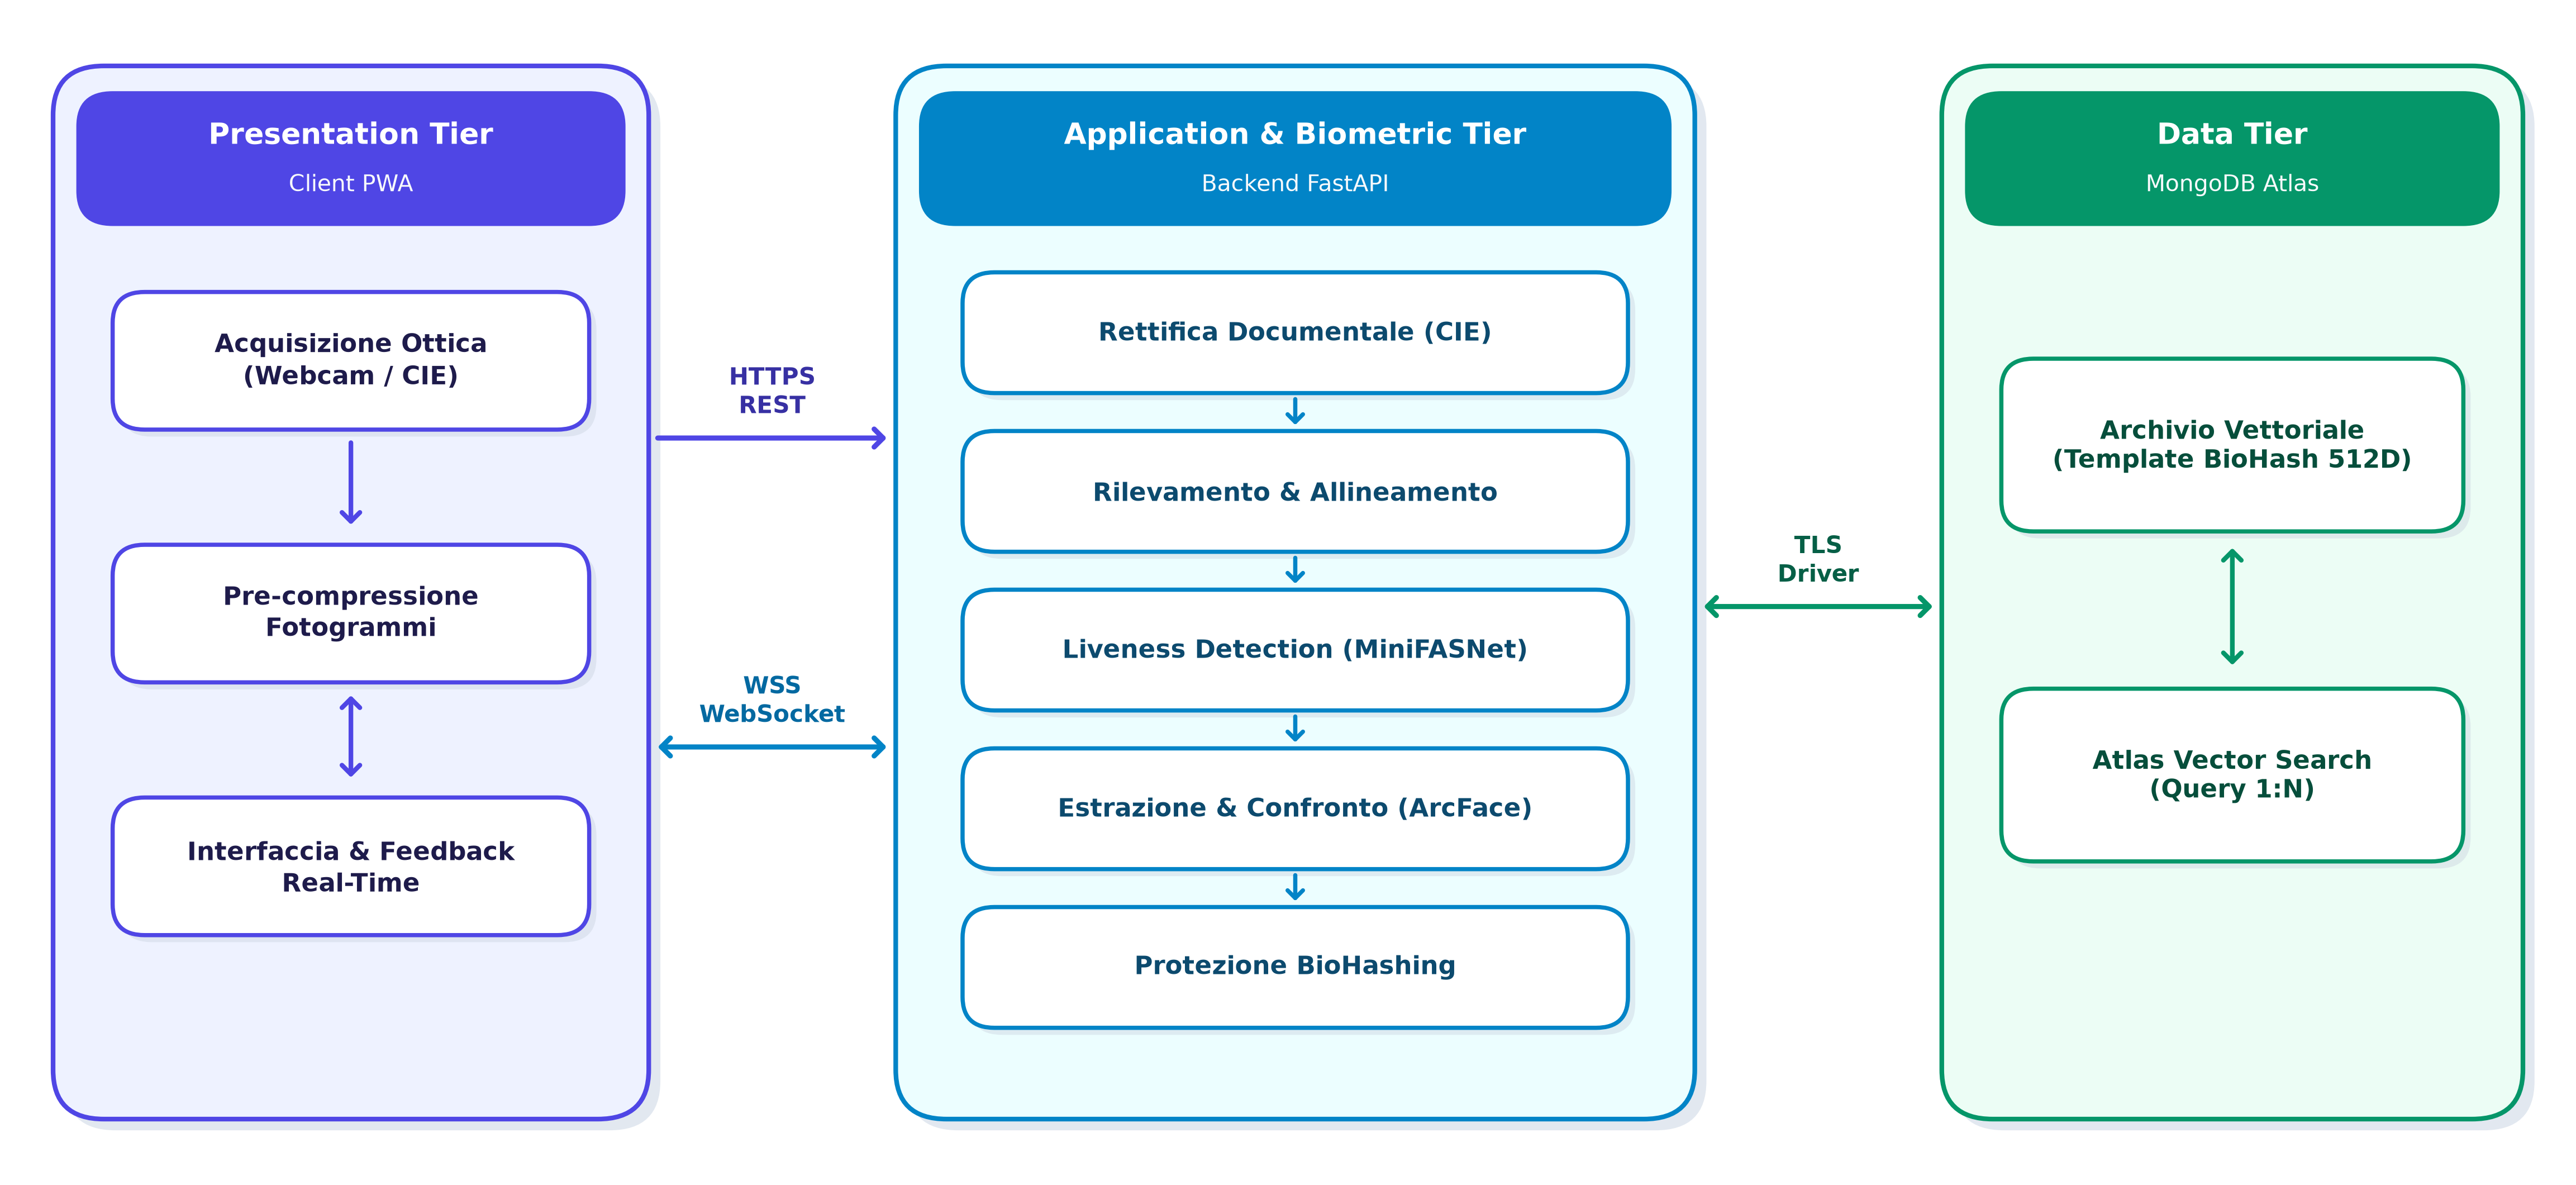
\includegraphics[width=1\linewidth]{images/diagramma-componenti.png}
    \caption{Architettura logica a tre livelli (\textit{Three-Tier Architecture}) del sistema progettato}
    \label{fig:diagrammaComponenti}
\end{figure}
L'interazione tra il \textit{Presentation Tier} e l'\textit{Application Tier}, schematizzata nel diagramma dei componenti in Figura~\ref{fig:diagrammaComponenti}, adotta un'architettura protocollare ibrida interamente incapsulata su canali cifrati \textbf{TLS} (\textit{Transport Layer Security}), al fine di mitigare i rischi di intercettazione (\textit{Man-in-the-Middle}) e manipolazione del traffico al livello L6 della tassonomia di esposizione (requisito $RNF5$).
A livello progettuale, la coerenza dei contratti di interfaccia tra client, server e database è garantita dall'adozione del pattern \textit{\gls{dto}} implementato mediante schemi formali di validazione che impongono un controllo rigoroso dei tipi di dato (\textit{type-checking}), dei formati di file e dei limiti dimensionali su tutti i payload in ingresso e in uscita.
La scelta del protocollo di trasporto al livello applicativo è stata differenziata in funzione della natura transazionale e dei vincoli di latenza dei due flussi operativi del sistema, le cui pipeline algoritmiche sono modellate in dettaglio nella Sezione~\ref{cap:2.3-pipeline}.
\begin{itemize}
    \item \textbf{Protocollo HTTPS REST} per il flusso di Enrollment (\texttt{POST /register}): poichè la registrazione di una nuova identità consiste in una transazione atomica e puntuale. Essa viene esposta tramite un architettura \textbf{RESTful sincrona su protocollo HTTPS}. L'interazione segue il classico paradigma \textit{request-response stateless}: il client invia una singola richiesta codificata in formato standard \texttt{multipart/form-data} che consente di trasmettere simultaneamente campi testuali (il nominativo completo dell'utente) e uno stream binario (la fotografia del documento d'identità). Il livello applicativo valida in RAM la conformità formale della richiesta (tipo MIME, integrità dell'immagine e dimensione massima di $5~\text{MB}$) e, una volta completata la pipeline di estrazione e indicizzazione, restituisce al client un oggetto strutturato in formato \texttt{JSON} accompagnato dal codice di stato semantico \texttt{HTTP 201 Created} in caso di successo, oppure un codice di errore \texttt{HTTP 4xx} in caso di rifiuto o violazione del vincolo di unicità $RF5$;
    \item \textbf{Protocollo \gls{wss}} per il flusso di Live Verification (\texttt{WSS /login}): poiché il processo di verifica in diretta richiede il trasferimento \textit{real-time} e a bassa latenza di una sequenza di fotogrammi dalla fotocamera del client verso il backend. Questo è utile per alimentare l'analisi temporale di vitalità e il matching biometrico (requisiti $RF3$ e $RF4$). L'adozione di richieste \texttt{HTTP/REST} tradizionali per trasmettere un flusso video ad alta frequenza ($15-30~\text{fps}$) risulterebbe architetturalmente proibitiva: la natura \textit{stateless} di HTTP imporrebbe, per ciascun fotogramma, la rinegoziazione degli header, la gestione di molteplici connessioni concorrenti e l'impossibilità per il server di mantenere in memoria lo stato della sessione. Per superare tale limite e soddisfare il requisito di bassa latenza ($RNF1$), la comunicazione è stata ingegnerizzata sul protocollo \textbf{WebSocket su canale sicuro (\gls{wss})}. Attraverso un singolo handshake iniziale HTTP \texttt{Upgrade} su TLS, il sistema instaura un canale TCP persistente, \textit{stateful} e bidirezionale (\textit{full-duplex}) a bassissimo overhead. Sul tunnel \gls{wss} viene inoltre adottata una strategia di serializzazione asimmetrica:
    \begin{itemize}
        \item in direzione \textbf{Client $\rightarrow$ Server}, i fotogrammi catturati dalla webcam vengono inviati come \textbf{frame binari puri} (\textit{binary payload}), evitando la codifica testuale in stringa \textit{Base64} che introdurrebbe un incremento di circa il $33\%$ sulla dimensione dei dati trasmessi e un costo aggiuntivo di serializzazione/deserializzazione~\cite{sawetsutipunFacialImageVerification2020a};
        \item in direzione \textbf{Server $\rightarrow$ Client}, il backend trasmette in modo asincrono messaggi testuali leggeri in formato \textbf{JSON}, notificando in tempo reale all'interfaccia grafica lo stato della sessione, le metriche parziali di avanzamento (requisito $RF6$) e il verdetto finale di autenticazione prima della chiusura controllata del socket.
    \end{itemize}
\end{itemize}
La Tabella~\ref{tab:confrontoFlussi} sintetizza il confronto architetturale e protocollare tra i due canali di comunicazione progettati.
\begin{table}[H]
    \centering
    \footnotesize
    \renewcommand{\arraystretch}{1.25}
    %\begin{tabular}{c c c c}
    \begin{tabular*}{\textwidth}{@{\extracolsep{\fill}} >{\raggedright\arraybackslash}p{3.2cm} >{\raggedright\arraybackslash}p{5.0cm} >{\raggedright\arraybackslash}p{5.2cm} @{}}
        \hline
        \textbf{Caratteristica} & \textbf{Enrollment (\texttt{/register})} & \textbf{Live Verification (\texttt{/login})} \\
        \hline
        \textbf{Paradigma e Protocollo} & \textit{Request-Response} sincrono su \textbf{HTTPS REST} (\texttt{POST}). & Canale persistente \textit{full-duplex} su \textbf{WebSocket Secure (\gls{wss})}. \\
        %\hline
        \textbf{Gestione dello Stato} & \textit{Stateless} (transazione atomica e indipendente). & \textit{Stateful} (mantenimento in RAM della sessione dell'utente). \\
        %\hline
        \textbf{Formato (Client $\rightarrow$ Server)} & Form-data (\texttt{multipart/form-data}): stringa nome completo + file immagine \gls{cie}. & Stream continuo di pacchetti binari puri (\texttt{bytes}) dei fotogrammi video. \\
        %\hline
        \textbf{Formato (Server $\rightarrow$ Client)} & Singolo payload \textbf{JSON} validato da \gls{dto} con esito e metadati (\texttt{HTTP 201}). & Flusso asincrono di messaggi \textbf{JSON} con avanzamento real-time e verdetto finale. \\
        %\hline
        \textbf{Overhead di Rete} & Standard HTTP/TLS (accettabile per transazione). & Minimizzato (singolo handshake iniziale, assenza di overhead). \\
        \hline
    %\end{tabular}
    \end{tabular*}
    \caption{Confronto architetturale e protocollare tra il flusso di registrazione (\textit{enrollment}) tramite \gls{cie} e il flusso di verifica biometrica in tempo reale.}
    \label{tab:confrontoFlussi}
\end{table}


%===============================================

\section{Modellazione delle pipeline e Macchina a Stati Finiti (FSM)}\label{cap:2.3-pipeline}
Definita l'infrastrutura Client-Server e i protocolli di trasporto, la progettazione si è concentrata sulla modellazione algoritmica dei due flussi opeativi principali del sistema: \textit{enrollment} e \textit{live verification}, governata da una \textbf{Macchina a Stati Finiti (\gls{fsm})}.
Il flusso di \textit{enrollment}, innescato dalla chiamata sincrona \texttt{POST /register}, ha l'obiettivo di acquisire il lato anteriore di un documento conforme allo standard ICAO 9303 formato TD1 (come la \gls{cie} o la patente di guida italiana), normalizzarne le proprietà geometriche e prospettiche ed estrarre un template di riferimento univoco e protetto~\cite{icao9303,kelesRepublicTurkeyIdentity2020}. 
Alla chiamata dell'\textit{endpoint}, nel rispetto del vincolo $RNF2$, lo stream binario ricevuto nel payload \texttt{multipart/form-data} viene decodificato direttamente in memoria volatile (RAM) come matrice numerica multibanda e attraversa i cinque stadi sequenziali descritti nel Capitolo~\ref{cap:2.2-architettura}. In particolare nel modulo di \textbf{rettifica documentale} l'immagine viene sottoposta a una serie di operazioni, per correggere le inevitabili rotazioni e distorsioni prospettiche, essendo acquisita a mano libera dall'utente in condizioni non vincolate:
\begin{enumerate}
    \item \textbf{Conversione in scala di grigi e applicazione di un filtro di \textit{Gaussian Blur}} per ridurre il rumore e le texture non uniformi. Permette di individuare meglio i gradienti dei bordi mediante l'algoritmo di \textit{Canny Edge Detection};
    \item \textbf{Analisi topologica dei contorni e approssimazione poligonale} tramite algoritmo di \textit{Douglas-Peucker}: si isola il quadrilatero di area massima corrispondente ai quattro vertici fisici della tessera sfruttando le dimensioni fisiche nominali del formato ID-1 / ICAO TD1 ($85{,}6 \times 54{,}0~\text{mm}$), caratterizzato da un \textit{aspect ratio} di $85{,}6/54{,}0 \approx 1{,}58$~\cite{icao9303};
    \item \textbf{Calcolo della matrice di omografia planarizzata} $H$ che mappa i vertici rilevati ai vertici di un rettangolo standard $856 \times 540$ pixel e applicazione della trasformazione prospettica (\textit{warp perspective}) per ottenere un'immagine rettificata e allineata;
    \item \textbf{Equalizzazione adattiva del contrasto (\gls{clahe})} per mitigare la compressione tonale, i riflessi olografici sul policarbonato e la bassa risoluzione della fototessera stampata. In particolare, l'algoritmo \gls{clahe} viene applicato solo sul canale di luminanza $L$: 
    \begin{itemize}
        \item Suddivisione l'immagine in blocchi locali
        \item Calcolo dell'istogramma di luminanza di ciascun blocco
        \item Applicazione di una limitazione del contrasto per evitare l'amplificazione del rumore, migliorando la leggibilità dei dettagli del volto
    \end{itemize}
\end{enumerate}
L'immagine rettificata e migliorata, viene quindi passata al modulo di \textbf{rilevamento e allineamento facciale}, il quale:
\begin{enumerate}
    \item \textbf{Intervento del rilevatore facciale} per localizzare il \textit{bounding box} del volto della fototessera ed estrarre le coordinate bidimensionali dei 5 \textit{keypoint biometrici} ${(x_k, y_k)}_{k=1}^{5}$ (centri oculari, punta del naso e angoli labiali);
    \item \textbf{Estrazione del volto più grande} valutando l'area del \textit{bounding box}
    \item \textbf{Allineamento geometrico} mediante trasformazione affine, normalizzando la dimensione a $112 \times 112$ pixel;
\end{enumerate}
Successivamente, il volto con i keypoint allineati viene passato al modulo di \textbf{estrazione e confronto}, che con la rete \textit{ResNet-100} (\texttt{buffalo\_l}) processa il tensore $112 \times 112 \times 3$ e genera un embedding $e \in \mathbb{R}^{512}$ normalizzato ($\lVert e \rVert_2 = 1$) come specificato nel Capitolo~\ref{cap:1-fondamenti}~\cite{dengArcFaceAdditiveAngular2022}.
Prima di procedere alla registrazione, per soddisfare il requisito di unicità ($RF5$) conforme alle specifiche di \textit{identification} ICAO 9303~\cite{icao9303}, il backend esegue una query vettoriale $1:N$ sull'indice \textit{MongoDB Atlas Vector Search} confrontando $e_{\text{ID}}$ con tutti i template già registrati nel database attraverso la \textit{Cosine Similarity}.
Qualora il punteggio massimo di \textit{similarità coseno} superi la soglia decisionale, ovvero $\max_{j} S_c(e_{\text{ID}}, e_j) \ge \tau$, la transazione viene interrotta restituendo un errore semantico \texttt{HTTP 409 Conflict} al client, notificando che il soggetto biometrico è già registrato. In caso contrario, il vettore $e_{\text{ID}}$ viene protetto con la trasformazione di \textit{biohashing} descritta nel capitolo~\ref{cap:1.4-normative}, a partire da un seme crittografico casuale $K$ specifico dell'utente, producendo il template binario irreversibile $c_{\text{ID}} \in {\{0, 1\}}^m$ che viene indicizzato nel database insieme al nominativo dell'utente, al seed e al \textit{timestamp} di creazione.
Invece le matrici d'immagine del documento e del ritaglio facciale vengono immediatamente deallocate dalla RAM ed eliminate.
In figura~\ref{fig:diagrammaSequenzaRegistrazione} è riportato il diagramma di sequenza UML che modella l'interazione temporale tra i componenti durante la pipeline di \textit{enrollment}.
\begin{figure}[H]
    \centering
    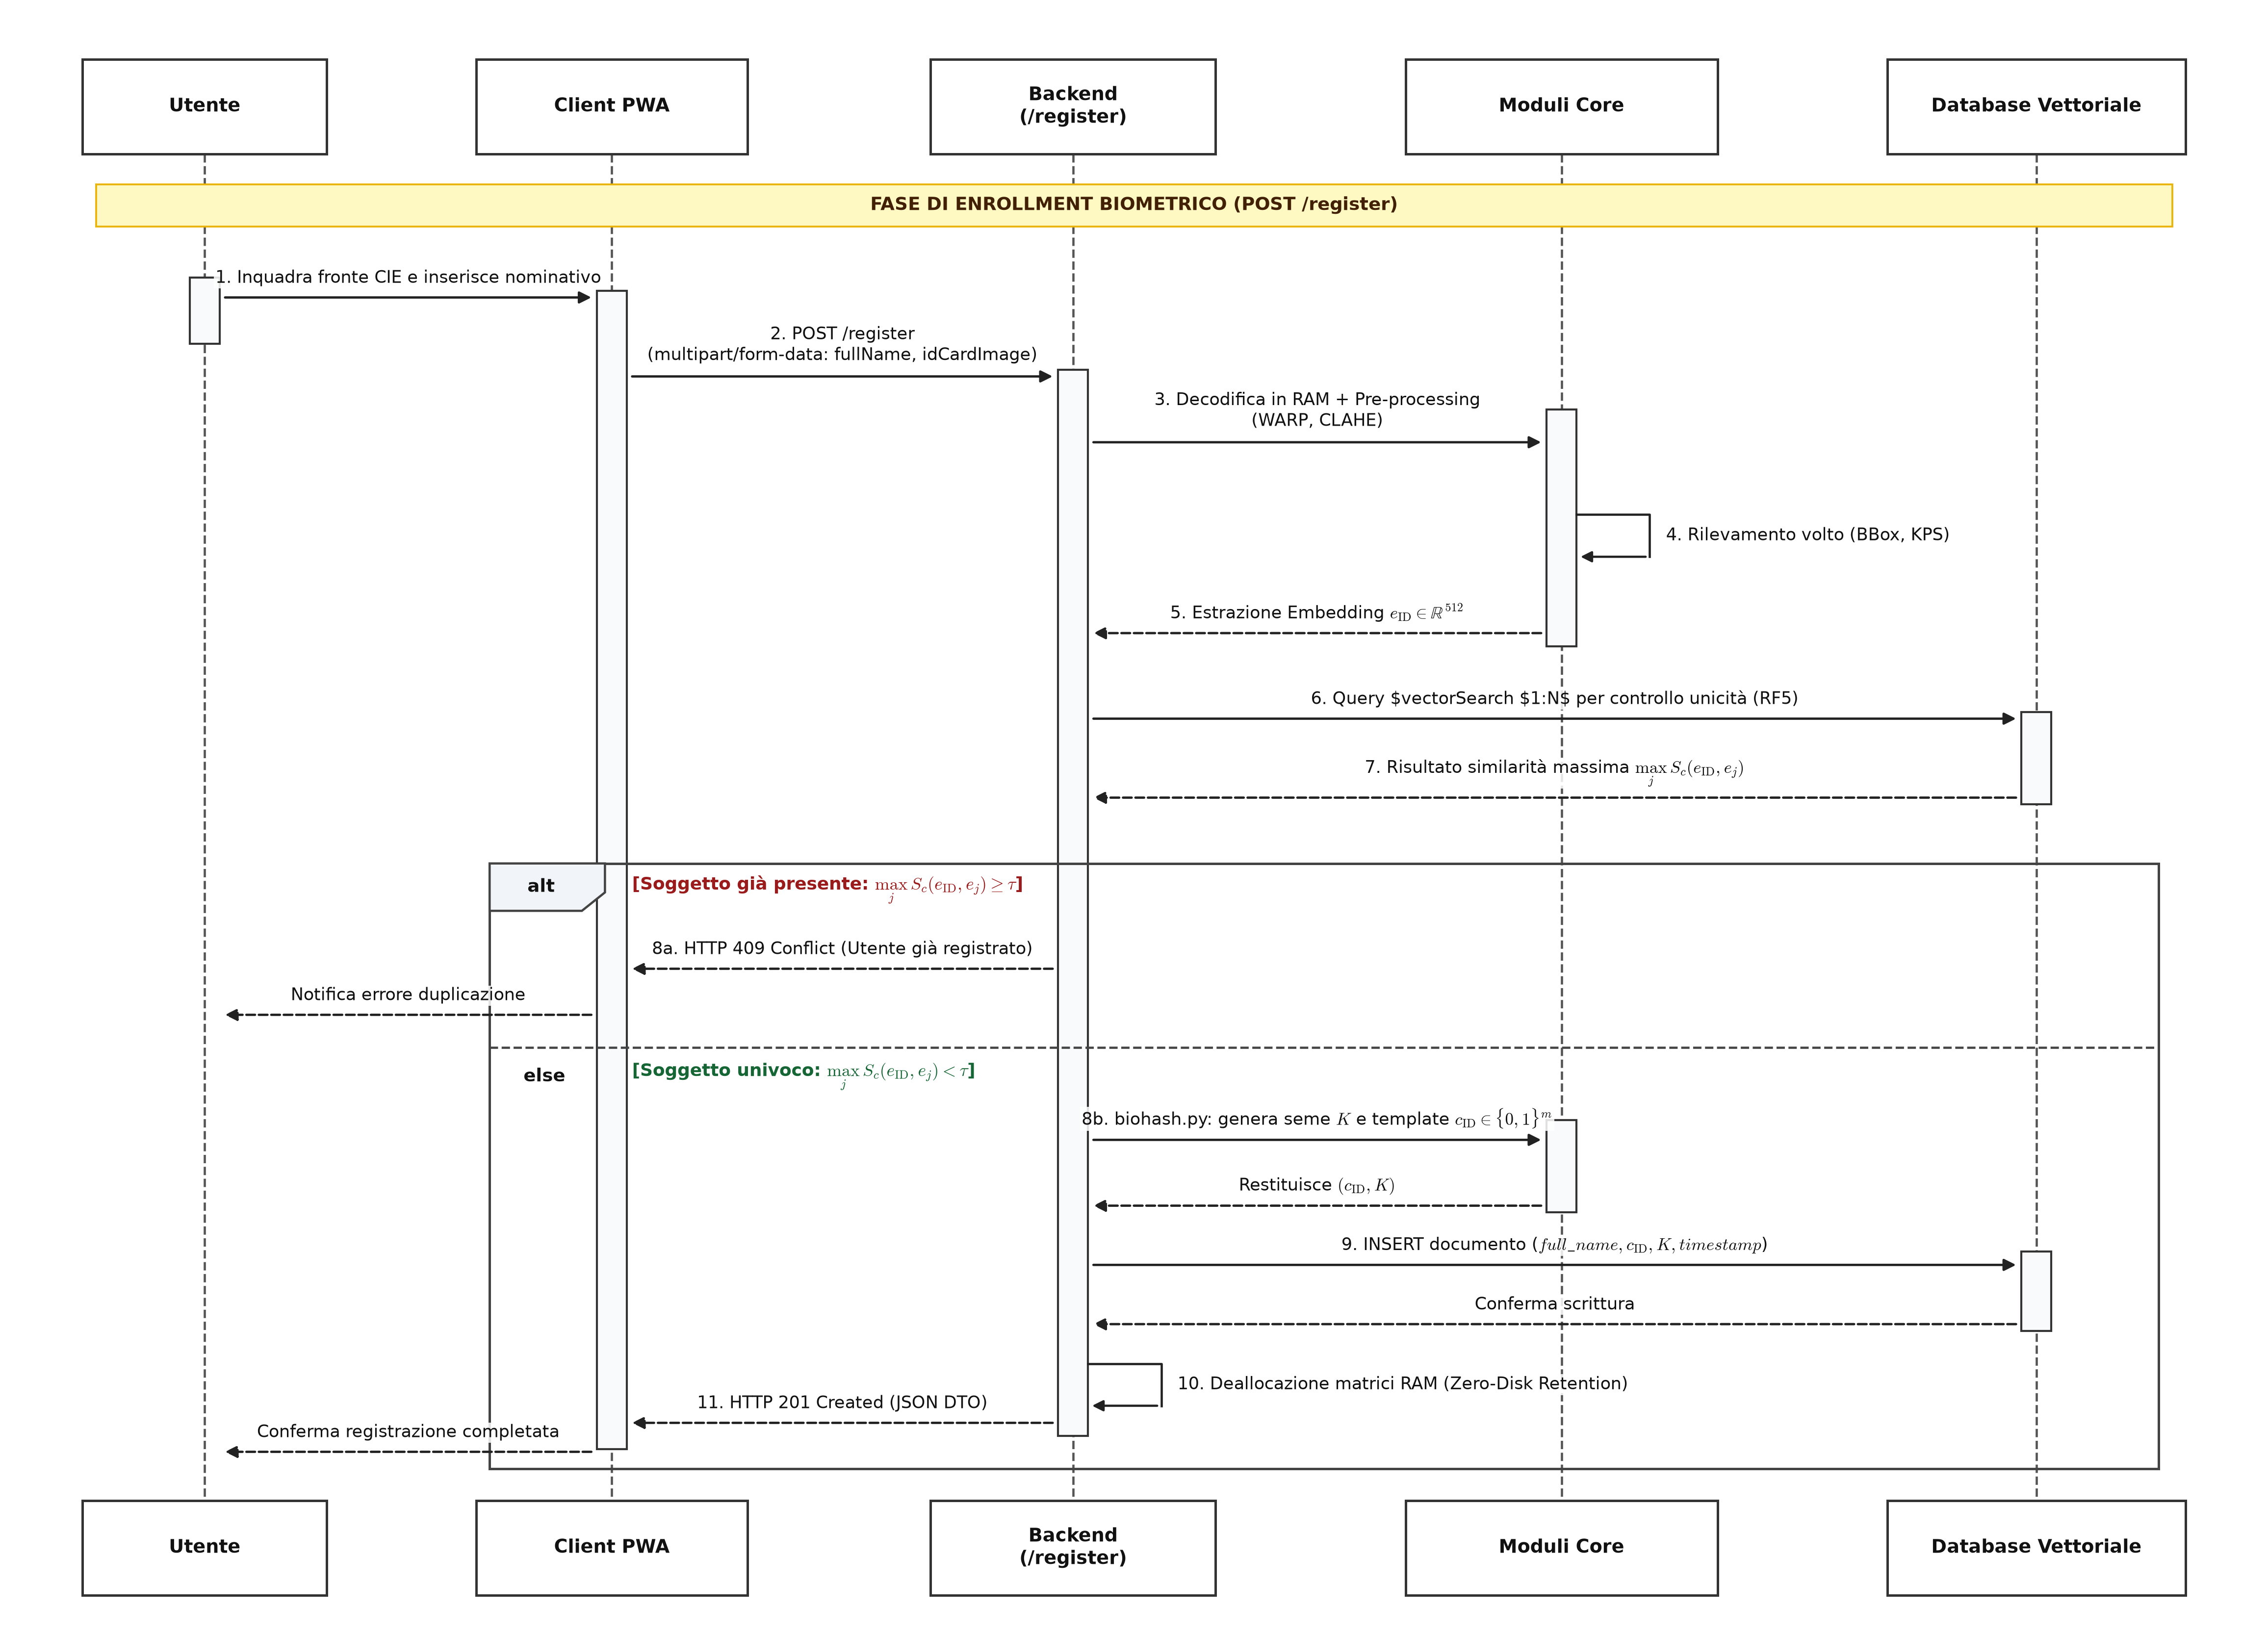
\includegraphics[width=\linewidth]{images/diagrammaSequenza-Registrazione.png}
    \caption{Diagramma di sequenza UML della pipeline di \textit{enrollment} tramite \gls{cie}}
    \label{fig:diagrammaSequenzaRegistrazione}
\end{figure}
Una volta registrato il template, e indicizzata la nuova identità, l'utente può accedere al flusso di autenticazione in diretta (\textit{live verification}) tramite il canale \gls{wss} persistente.
Come evidenziato nell'analisi delle criticità (Capitolo~\ref{cap:2.1-criticita}), il flusso di \textit{live verification} richiede un'elaborazione in tempo reale di più fotogrammi per valutare la presenza biologica reale dell'utente, evitando l'instabilità dovuta ad artefatti di \textit{motion blur}, variazioni di illuminazione o \textit{pose} estreme o attacchi \gls{pa}~\cite{liSilentFaceAntiSpoofing2024}.
Per garantire una valutazione spazio-temporale robusta ($RF3$ e $RF4$), il ciclo di vita di ciascuna connessione Websocket è governato sul server da una \textbf{Macchina a Stati Finiti (\gls{fsm})} deterministica, formalmente definita dalla quintupla nella equazione~\ref{eq:fsm}~\cite{sommerville2015software, hopcroftIntroductionAutomataTheory2007a}:
\begin{equation}
    \label{eq:fsm}
    \mathcal{M} = (\Sigma, \, S, \, s_0, \, \delta, \, F)
\end{equation}
dove:
\begin{itemize}
    \item $\Sigma$ è l'insieme degli input, generati dall'analisi di ciascun fotogramma binario $f_t$ ricevuto all'istante $t$: \begin{itemize}
        \item presenza/assenza del volto
        \item conteggio del buffer $n$
        \item punteggio di vitalità $l_t$
        \item percentuali di spoofing con \gls{pa} ${\%_{\text{\gls{pa}}}}_t$ (\textit{print attack}, \textit{replay attack})
        \item punteggio di qualità ${q_{\text{face}}}_t$
        \item punteggio di similarità ${S_c}_t$
        \item varianza geometrica dei keypoint $\sigma_{\text{kps}}^2$
    \end{itemize}
    \item $S$ è l'insieme degli stati:\begin{itemize}
        \item \texttt{WAITING\_FACE}
        \item \texttt{WAITING\_LIVENESS}
        \item \texttt{SPOOF\_ATTACK}
        \item \texttt{MATCH} o \texttt{NO\_MATCH}
    \end{itemize}
    \item $s_0$ è lo stato iniziale all'apertura dell'handshake: \texttt{WAITING\_FACE};
    \item $\delta$ è la funzione di transizione di stato: $S \times \Sigma \rightarrow S$;
    \item $F$ è l'insieme degli stati finali: $\{\texttt{SPOOF\_ATTACK}, \, \texttt{MATCH / NO\_MATCH}\}$
\end{itemize}
Il funzionamento algoritmico della pipeline di autenticazione si sviluppa attraverso l'evoluzione sequenziale degli stati di $\mathcal{M}$.
\begin{enumerate}
    \item \textbf{Stato $s_0$ \texttt{WAITING\_FACE}}: il server riceve i fotogrammi binari $f_t$ dal client e li passa al modulo di \textit{rilevamento facciale}. Se il volto non viene rilevato, la macchina rimane in questo stato, notificando al client di posizionarsi frontalmente. Se il volto viene rilevato, si passa allo stato successivo $s_1$ \texttt{WAITING\_LIVENESS}, inizializzando in RAM le strutture dati del buffer temporale.
    \item \textbf{Stato $s_1$ \texttt{WAITING\_LIVENESS}}: rappresenta il nucleo dell'analisi temporale multi-frame, progettato per raccogliere una finestra di $N$ fotogrammi consecutivi (con $N \in [30,60]$ corrispondenti a circa $1\sim2~\text{secondi}$ di acquisizione video). Per ogni fotogramma ricevuto $f_t~\text{con}~t \in \{1, \dots, N\}$, il backend esegue le seguenti operazioni in tempo reale: \begin{enumerate}
        \item Calcola lo \textbf{score di vitalità passiva} $l_t$ con \textit{MiniFASNet} su \gls{onnx} Runtime, accumulando nel vettore di sessione $\mathbf{l} = [l_1, \dots, l_N]$;
        \item \textbf{Aggiorna il contatore} $p$ dei tentativi di spoofing se dall'analisi del frame $f_t$ risultano percentuali sopra soglia ($\tau_{\text{live}}$) di \textit{print attack} o \textit{replay attack}
        \item Registra la posizione dei \textbf{5 keypoint biometrici} ${(x_{k,t}, y_{k,t})}_{k=1}^{5}$ per monitorarne la micro-varianza spaziale $\sigma_{\text{kps}}^2$ nel tempo, assicurandosi che il soggetto presenti una naturale vitalità biologica ma mantenga una posa frontale neutra conforme ai limiti angolari ($\pm 15^\circ$) dello standard ICAO 9303~\cite{icao9303};
        \item Aggiorna il riferimento al \textbf{fotogramma ottimo} trattenendo in memoria il frame caratterizzato dal punteggio di rilevamento e nitidezza ottica più alto $f_{\text{best}} = \arg\max_{t} {q_{\text{face}}}_t$;
        \item \textbf{Invia al client} un messaggio \texttt{JSON} con la percentuale di avanzamento del buffer $\text{progress} = \frac{t}{N} \cdot 100$ per aggiornare la barra di stato nella \gls{pwa} (rispettando il requisito $RF6$).
    \end{enumerate}
    Qualora l'utente esca dall'inquadratura prima del completamento del buffer, la \gls{fsm} azzera l'accumulatore e riporta la sessione in $s_0$.
    Al raggiungimento degli $N$ fotogrammi ($t = N$), la macchina valuta lo score medio di vitalità $\bar{l}$ e la micro-varianza dei keypoint attraverso la condizione di vitalità congiunta definita nell'Equazione~\eqref{eq:criterioLivenessBuffer}:
    \begin{equation}
        \label{eq:criterioLivenessBuffer}
        \bar{L} = \frac{1}{N} \sum_{t=1}^{N} l_t \ge \tau_{\text{liveness}} \quad \land \quad \sigma_{\text{kps}}^2 \in [\sigma_{\min}^2, \, \sigma_{\max}^2]
    \end{equation}
    dove $\bar{L}$ è la media aritmetica degli score passivi (con soglia $\tau_{\text{liveness}} = 0{,}50$) e $[\sigma_{\min}^2, \, \sigma_{\max}^2]$ delimita l'intervallo di micro-movimento fisiologico dei \textit{landmark} (escludendo sia la rigidità assoluta di una foto fissa sia movimenti bruschi che causano \textit{motion blur});

    \item \textbf{Stato $s_2$ \texttt{SPOOF\_ATTACK}}: si finisce in questo stato se al termine della valutazione del buffer (o anticipatamente in presenza di $M$ frame fortemente negativi), risulta $\bar{L} < \tau_{\text{liveness}}$ oppure $\sigma_{\text{kps}}^2 < \sigma_{\min}^2$. Il server blocca l'esecuzione del modulo di riconoscimento facciale, notifica al frontend il tentativo di \textit{spoofing} e dealloca il buffer dalla RAM;

    \item \textbf{Stato $s_3$ \texttt{MATCH / NO\_MATCH}}: se la condizione di vitalità è soddisfatta, il backend esegue il modulo di estrazione e confronto sul fotogramma ottimo $f_{\text{best}}$, calcolando l'embedding $e_{\text{live}} \in \mathbb{R}^{512}$ tramite \textit{\gls{arcface}} e lancia \textbf{una singola query vettoriale $1:N$} su \textit{MongoDB Atlas Vector Search}. 
    Ricevuto il candidato più vicino dal database con score di similarity coseno $S_c(e_{\text{live}}, e_{\text{ID}})$, ed effettuata la verifica di coerenza sul template protetto tramite \textit{BioHashing} con il seme $K$ associato~\cite{otroshishahrezaBenchmarkingCancelableBiometrics2022}, il sistema applica la regola decisionale rispetto alla soglia calibrata $\tau \in [0{,}30, \, 0{,}50]$ ($RF4$).
    Se $S_c \ge \tau$, l'identità viene confermata (\texttt{MATCH}) restituendo al client i dati dell'utente autenticato; se $S_c < \tau$, l'accesso viene respinto (\texttt{NO\_MATCH}).
    In entrambi i casi, il buffer viene distrutto dalla memoria volatile ($RNF2$) e la sessione WebSocket viene chiusa in modo controllato.
\end{enumerate}
La Tabella~\ref{tab:statiFSM} riassume formalmente gli stati della \gls{fsm} progettata, mentre la Figura~\ref{fig:diagrammaSequenza-login} illustra il diagramma di sequenza UML dell'intero ciclo di verifica su WebSocket.
\begin{figure}[H]
    \centering
    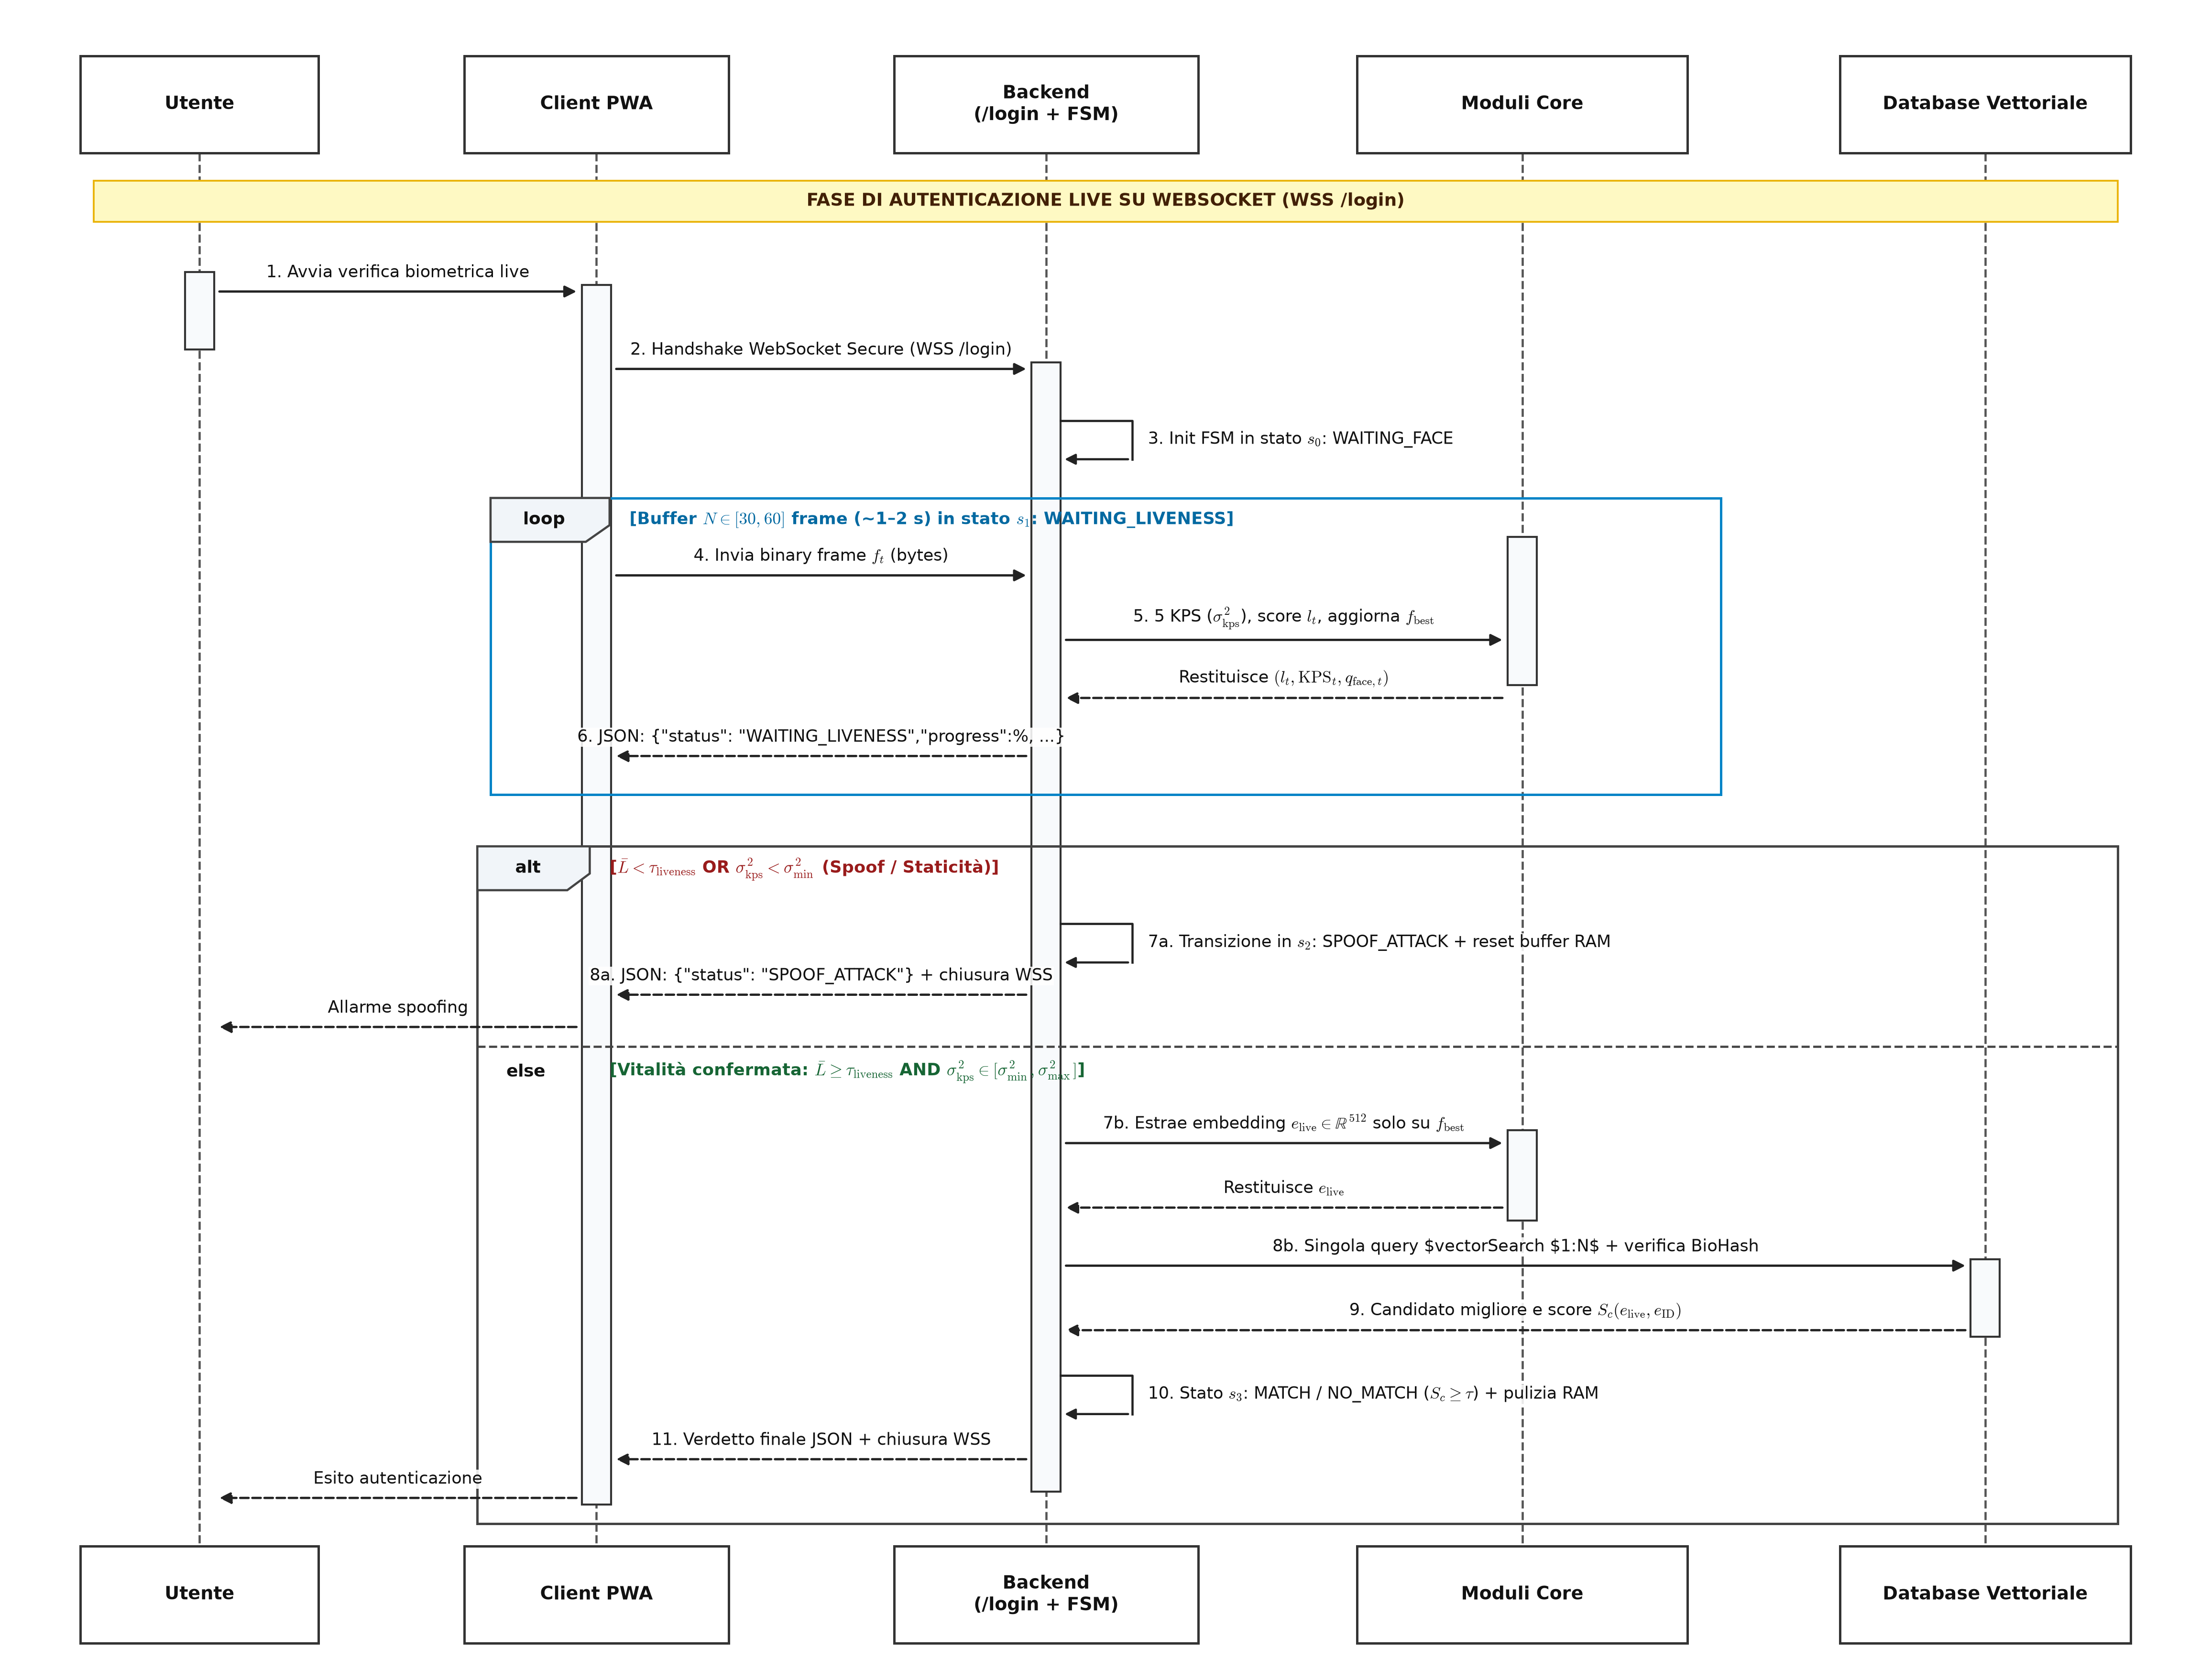
\includegraphics[width=\linewidth]{images/diagrammaSequenza-Login.png}
    \caption{Diagramma di sequenza UML del flusso di autenticazione biometrica in tempo reale su (\texttt{WSS /login}) governato dalla Macchina a Stati Finiti ($\mathcal{M}$)}
    \label{fig:diagrammaSequenza-login}
\end{figure}

\begin{table}[H]
    \centering
    \footnotesize
    \renewcommand{\arraystretch}{1.25}
    %\begin{tabular}{c c c c}
    \begin{tabular*}{\textwidth}{@{\extracolsep{\fill}} >{\raggedright\arraybackslash}p{3.4cm} >{\raggedright\arraybackslash}p{7.2cm} >{\raggedright\arraybackslash}p{3.4cm} @{}}
        \hline
        \textbf{Stato Corrente} & \textbf{Condizione di Guardia ($\Sigma$)} & \textbf{Stato Prossimo} \\
        \hline
        $s_0$: \texttt{WAITING\_FACE} & $n_{\text{faces}} = 1$ (volto rilevato) & $s_1$: \texttt{WAITING\_LIVENESS} \\
        \hline
        $s_1$: \texttt{WAITING\_LIVENESS} & $n_{\text{faces}} = 0$ (volto perso) & $s_0$: \texttt{WAITING\_FACE} \\
        \hline
        $s_1$: \texttt{WAITING\_LIVENESS} & $t < N \land f_t \text{ valido}$ & $s_1$: \texttt{WAITING\_LIVENESS} \\
        \hline
        $s_1$: \texttt{WAITING\_LIVENESS} & $t = N \land (\bar{L} < \tau_{\text{liveness}} \lor \sigma_{\text{kps}}^2 \notin [\sigma_{\min}^2, \sigma_{\max}^2])$ & $s_2$: \texttt{SPOOF\_ATTACK} \\
        \hline
        $s_1$: \texttt{WAITING\_LIVENESS} & $t = N \land \bar{L} \ge \tau_{\text{liveness}} \land \sigma_{\text{kps}}^2 \in [\sigma_{\min}^2, \sigma_{\max}^2] \land S_c(e_{\text{live}}, e_{\text{ID}}) \ge \tau$ & $s_3$: \texttt{MATCH} \\
        \hline
        $s_1$: \texttt{WAITING\_LIVENESS} & $t = N \land \bar{L} \ge \tau_{\text{liveness}} \land \sigma_{\text{kps}}^2 \in [\sigma_{\min}^2, \sigma_{\max}^2] \land S_c(e_{\text{live}}, e_{\text{ID}}) < \tau$ & $s_3$: \texttt{NO\_MATCH} \\
        \hline
    %\end{tabular}
    \end{tabular*}
    \caption{Tabella formale delle transizioni di stato della \gls{fsm} per la sessione di \textit{live verification}.}
    \label{tab:statiFSM}
\end{table}\newpage


L'adozione congiunta della pre-allocazione dei modelli neurali in memoria RAM (requisito $RNF1$) e della selezione del fotogramma ottimo all'interno della \gls{fsm}, consente di modellare rigorosamente il guadagno prestazionale del sistema rispetto all'architettura pregressa.
In un sistema \textit{stateless} non ottimizzato, che ricarica i pesi da disco ed esegue l'intera catena di estrazione ad ogni chiamata, il tempo di elaborazione per singolo fotogramma è stimabile dall'Equazione~\eqref{eq:latenzaSingoloFrame}:
\begin{equation}
    \label{eq:latenzaSingoloFrame}
    T_{\text{frame}} = \delta_{\text{cold}} \cdot T_{\text{load}} + T_{\text{det}} + T_{\text{pad}} + \delta_{\text{match}} \cdot (T_{\text{emb}} + T_{\text{db}})
\end{equation}
dove:
\begin{itemize}
    \item $T_{\text{load}}$ è il tempo di I/O per il caricamento in RAM dei grafi neurali ($\approx 3{-}4~\text{s}$);
    \item $T_{\text{det}}$ il tempo di rilevamento e allineamento sui 5 keypoint;
    \item $T_{\text{pad}}$ il tempo di inferenza di \textit{MiniFASNet} su \gls{onnx} Runtime;
    \item $T_{\text{emb}}$ il tempo di inferenza della backbone \textit{ResNet-100} (\texttt{buffalo\_l});
    \item $T_{\text{db}}$ la latenza di rete e ricerca su \textit{MongoDB Atlas};
    \item $\delta_{\text{cold}}, \delta_{\text{match}} \in \{0, 1\}$ sono coefficienti binari di attivazione. 
\end{itemize}
Grazie alla pre-allocazione dei modelli in RAM all'avvio del server (che impone $\delta_{\text{cold}} = 0$ per tutte le richieste utente) e al disaccoppiamento operato dalla \gls{fsm} tra lo stato iterativo $s_1$ ($\delta_{\text{match}} = 0$ per tutti gli $N$ frame del buffer) e lo stato finale $s_3$ ($\delta_{\text{match}} = 1$ una sola volta sul frame $f_{\text{best}}$), la latenza per singolo fotogramma durante lo streaming si riduce  si riduce all'Equazione~\eqref{eq:latenzaFrameOttimizzata}:
\begin{equation}
    \label{eq:latenzaFrameOttimizzata}
    T_{\text{frame}} = T_{\text{det}} + T_{\text{pad}} \approx 30{-}50~\text{ms}
\end{equation}
E di conseguenza, il tempo computazionale complessivo $T_{\text{buffer}}$ richiesto dal backend per completare l'intera sessione di verifica su un buffer di $N$ fotogrammi è formalizzato nell'Equazione~\eqref{eq:latenzaTotaleBuffer}: 
\begin{equation}
    \label{eq:latenzaTotaleBuffer}
    T_{\text{buffer}} = \sum_{t=1}^{N} \left( T_{\text{det}, t} + T_{\text{pad}, t} \right) + T_{\text{emb}}(f_{\text{best}}) + T_{\text{db}}\\ \approx N \cdot (\bar{T}_{\text{det}} + \bar{T}_{\text{pad}}) + T_{\text{emb}} + T_{\text{db}}
\end{equation}
Abbattendo in questo modo la complessità delle operazioni più onerose ($T_{\text{emb}}$ e $T_{\text{db}}$) da $\mathcal{O}(N)$ a $\mathcal{O}(1)$ per sessione di login. L'architettura riesce a mantenere il frame rate di acquisizione fluido ($\sim 20{-}30~\text{fps}$) e restituisce il verdetto di autenticazione entro una finestra sub-secondo dal completamento del buffer video.
%TODO: in caso di connessioni instabili (mobile)

% Pipeline di enrollment e di verifica; Specifica formale della FSM di sessione
% 5pp

%===============================================

\section{Persistenza vettoriale e Stack Tecnologico}\label{cap2.4-persistenza}
Modello dati MongoDB e ricerca HNSW (\$vectorSearch); Stack backend/frontend e gestione del ciclo di vita
4pp